\documentclass[12pt,letterpaper]{article}
\usepackage[utf8]{inputenc}
\usepackage[spanish]{babel}
\usepackage{graphicx}
\usepackage[left=2cm,right=2cm,top=2cm,bottom=2cm]{geometry}
\usepackage{graphicx} % figuras
% \usepackage{subfigure} % subfiguras
\usepackage{float} % para usar [H]
\usepackage{amsmath}
%\usepackage{txfonts}
\usepackage{stackrel} 
\usepackage{multirow}
\usepackage{enumerate} % enumerados
\renewcommand{\labelitemi}{$-$}
\renewcommand{\labelitemii}{$\cdot$}
% \author{}
% \title{Caratula}
\begin{document}

% Fancy Header and Footer
% \usepackage{fancyhdr}
% \pagestyle{fancy}
% \cfoot{}
% \rfoot{\thepage}
%

% \usepackage[hidelinks]{hyperref} % CREA HYPERVINCULOS EN INDICE

% \author{}
\title{Caratula}

\begin{titlepage}
\begin{center}
\large{UNIVERSIDAD PRIVADA-DE-TACNA}\\
\vspace*{-0.025in}
\begin{figure}[htb]
\begin{center}

\includegraphics[width=8cm]{./Imagenes/logo}
\end{center}
\end{figure}
\vspace*{0.15in}
INGENIERIA DE SISTEMAS  \\

\vspace*{0.5in}
\begin{large}
TITULO:\\
\end{large}

\vspace*{0.1in}
\begin{Large}
\textbf{INFORME DE LABORATORIO No 01} \\
\end{Large}

\vspace*{0.3in}
\begin{Large}
\textbf{CURSO:} \\
\end{Large}

\vspace*{0.1in}
\begin{large}
BASE DE DATOS II\\
\end{large}

\vspace*{0.3in}
\begin{Large}
\textbf{DOCENTE(ING):} \\
\end{Large}

\vspace*{0.1in}
\begin{large}
 Patrick Cuadros Quiroga\\
\end{large}

\vspace*{0.2in}
\vspace*{0.1in}
\begin{large}
Integrantes: \\
\begin{flushleft}
Orlando Antonio Acosta Ortiz		\hfill	(2015052775) \\
Orestes Ramirez Ticona              \hfill  (2015053236) \\
Nilson Laura Atencio     			\hfill 	(2015053846) \\
Roberto Zegarra Reyes 				\hfill 	(2010036175) \\
Richard Cruz Escalante 				\hfill 	(2013047247) \\
\end{flushleft}
\end{large}
\end{center}

\end{titlepage}


\tableofcontents % INDICE
\thispagestyle{empty} % INDICE SIN NUMERO
\newpage
\setcounter{page}{1} % REINICIAR CONTADOR DE PAGINAS DESPUES DEL INDICE

\section{INFORMACIÓN GENERAL} 

\begin{itemize}
\subsection{Objetivos:}
	\item Conocer los fundamentos del servicio REST Web Api.
	\item Saber usar los controladores usando Entity Framework.
	\item Poder intercambiar datos a la base de datos con el formato JSON usando Postman.

\subsection{Equipos, materiales, programas y recursos utilizados:}
	\item Computadora con sistema operativo Windows 10.
	\item Microsoft Visual Studio 2017
	\item Postman 7.0.7 para (x86) o (x64)


\end{itemize}
\section{MARCO TEORICO} 
\begin{itemize}
\subsection{Postman:}
	\item Gestiona y construye tus APIs rápidamente,Postman surgió originariamente como una extensión para el navegador Google Chrome. A día de hoy dispone de aplicaciones nativas para MAC y Windows y están trabajando en una aplicación nativa para Linux (disponible en versión beta).
	\item Está compuesto por diferentes herramientas y utilidades gratuitas (en la versión free) que permiten realizar tareas diferentes dentro del mundo API REST: creación de peticiones a APIs internas o de terceros, elaboración de tests para validar el comportamiento de APIs, posibilidad de crear entornos de trabajo diferentes (con variables globales y locales), y todo ello con la posibilidad de ser compartido con otros compañeros del equipo de manera gratuita (exportación de toda esta información mediante URL en formato JSON).
	\item Además, dispone de un modo cloud colaborativo (de pago) para que equipos de trabajo puedan desarrollar entre todos colecciones para APIs sincronizadas en la nube para una integración más inmediata y sincronizada.

\subsection{JSON :}
	\item Es un formato de texto sencillo para el intercambio de datos. 
          \item  Está constituído por dos estructuras:
Una colección de pares de nombre/valor. En varios lenguajes esto es conocido como un objeto, registro, estructura, diccionario, tabla hash, lista de claves o un arreglo asociativo.
Una lista ordenada de valores. En la mayoría de los lenguajes, esto se implementa como arreglos, vectores, listas o sequencias.
\subsection{API REST :}
          \item El término REST (Representational State Transfer) se originó en el año 2000, descrito en la tesis de Roy Fielding, padre de la especificación HTTP. Un servicio REST no es una arquitectura software, sino un conjunto de restricciones con las que podemos crear un estilo de arquitectura software, la cual podremos usar para crear aplicaciones web respetando HTTP. 

\end{itemize}
\subsection{CARACTERISTICAS DE API REST:}
 Las operaciones más importantes que nos permitirán manipular los recursos son cuatro.
 GET para consultar y leer, POST para crear, PUT para editar y DELETE para eliminar.

 El uso de hipermedios (término que en el ámbito de las páginas web define el conjunto de procedimientos para crear contenidos que contengan texto, imagen, vídeo, audio y otros métodos de información) para permitir al usuario navegar por los distintos recursos de una API REST a través de enlaces HTML.


\section{PROCEDIMIENTO} 
\begin{itemize}
	\item Paso 1: Abrir Visual Studio, Crear una solucion Web  [Aplicacion web ASP.NET(.NET Framework)]\\
		\begin{center}
		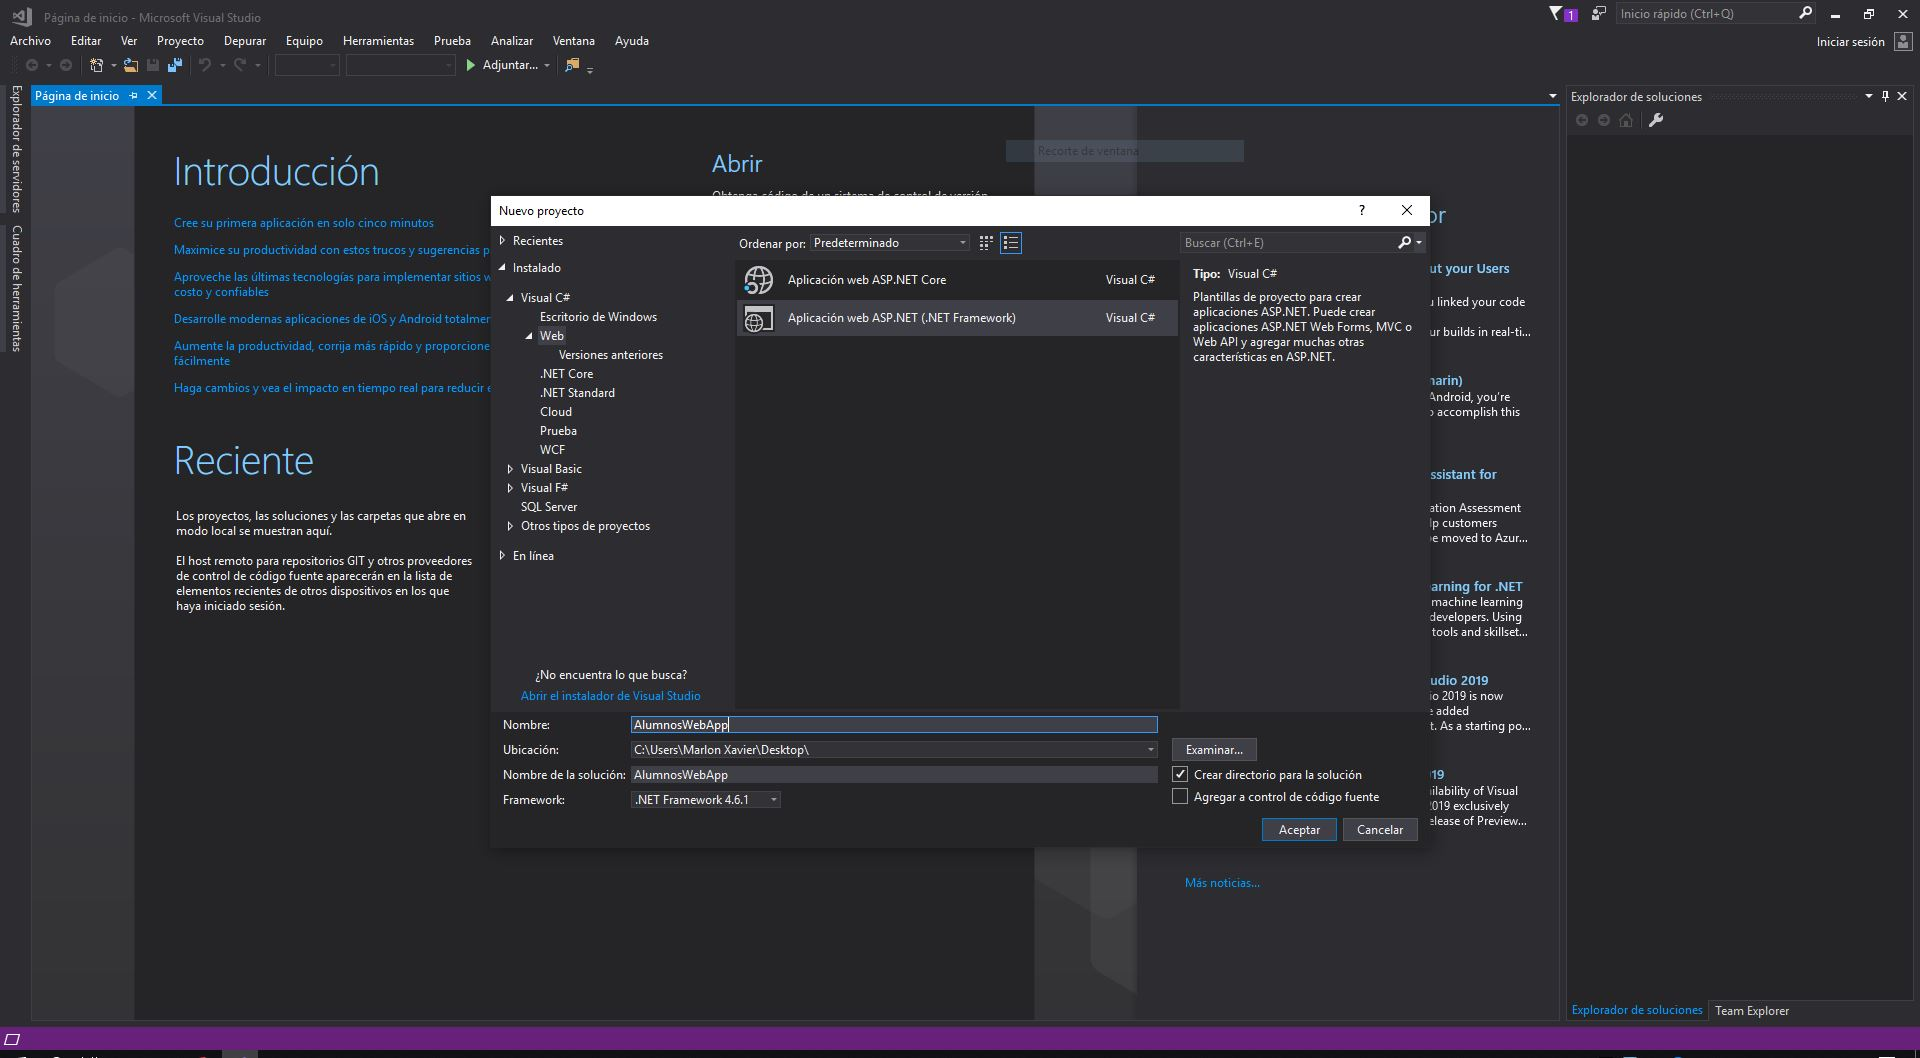
\includegraphics[width=15cm]{./Imagenes/Captura1}
		\end{center}
	\item Paso 2: Seleccionar la plantilla (Web API) con las opciones (MVC  y API web) marcadas\\
	\begin{center}
		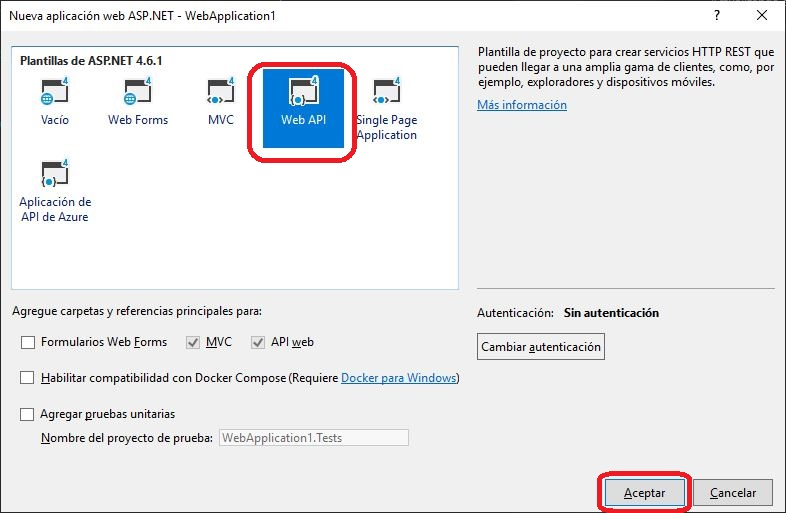
\includegraphics[width=15cm]{./Imagenes/Captura2}
		\end{center}
	\item Paso 3: Una vez creada la solución, dentro de la carpeta (Models)\\ Agregar 3 clases llamadas (Alumno, Tarea, TareaAlumno)\\
	\begin{center}
		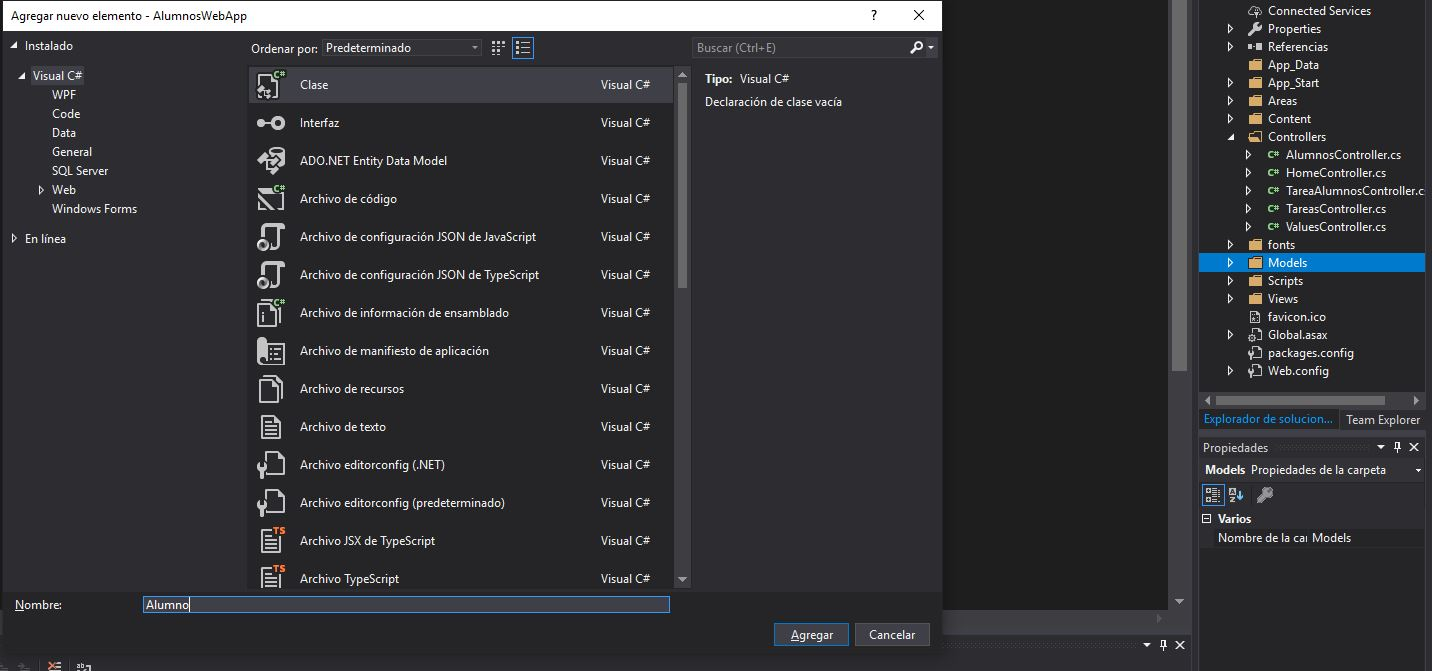
\includegraphics[width=15cm]{./Imagenes/Captura3}
		\end{center}
	\item Paso 4:Dentro de cada clase ingresar el codigo correspondiente a la siguiente imagen\\ (tener en cuenta agregar en la clase TareaAlumno:\\
	using System.Component.Model.DataAnnotations;\\
	using System.Component.Model.DataAnnotations.Schema;)\\
	\begin{center}
		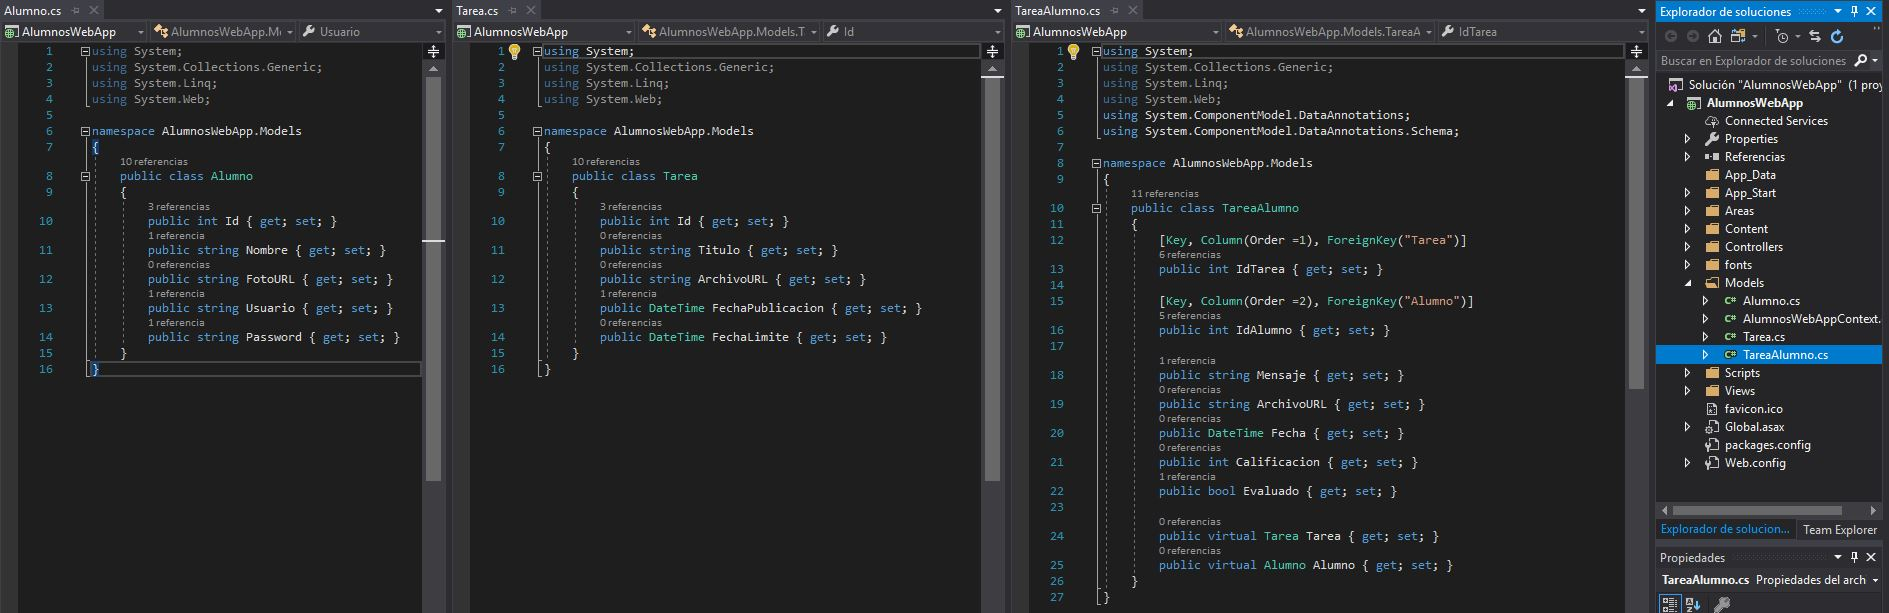
\includegraphics[width=15cm]{./Imagenes/Captura4}
		\end{center}
		\newpage
	\item Paso 5: Luego de terminar con las clases en Models, Pulsamos click derecho en la raiz de la solucion y por seguridad seleccionar las 3 primeras opciones(Para evitar errores al continuar con los siguientes pasos)\\
	\begin{center}
		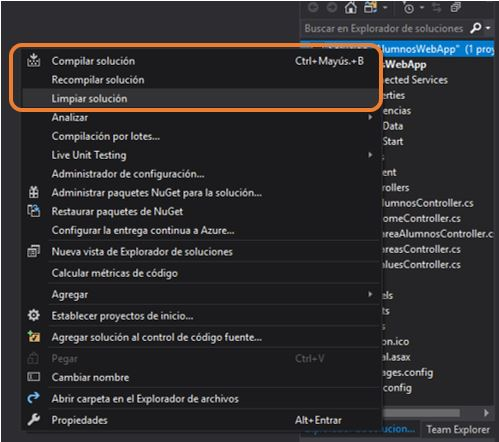
\includegraphics[width=15cm]{./Imagenes/Captura6}
	\end{center}
	\newpage
	\item Paso 6: Ahora hay que dirigirnos a la carpeta Controllers\\ 
	En la carpeta le damos a Agregar - Controlador\\
	\begin{center}
		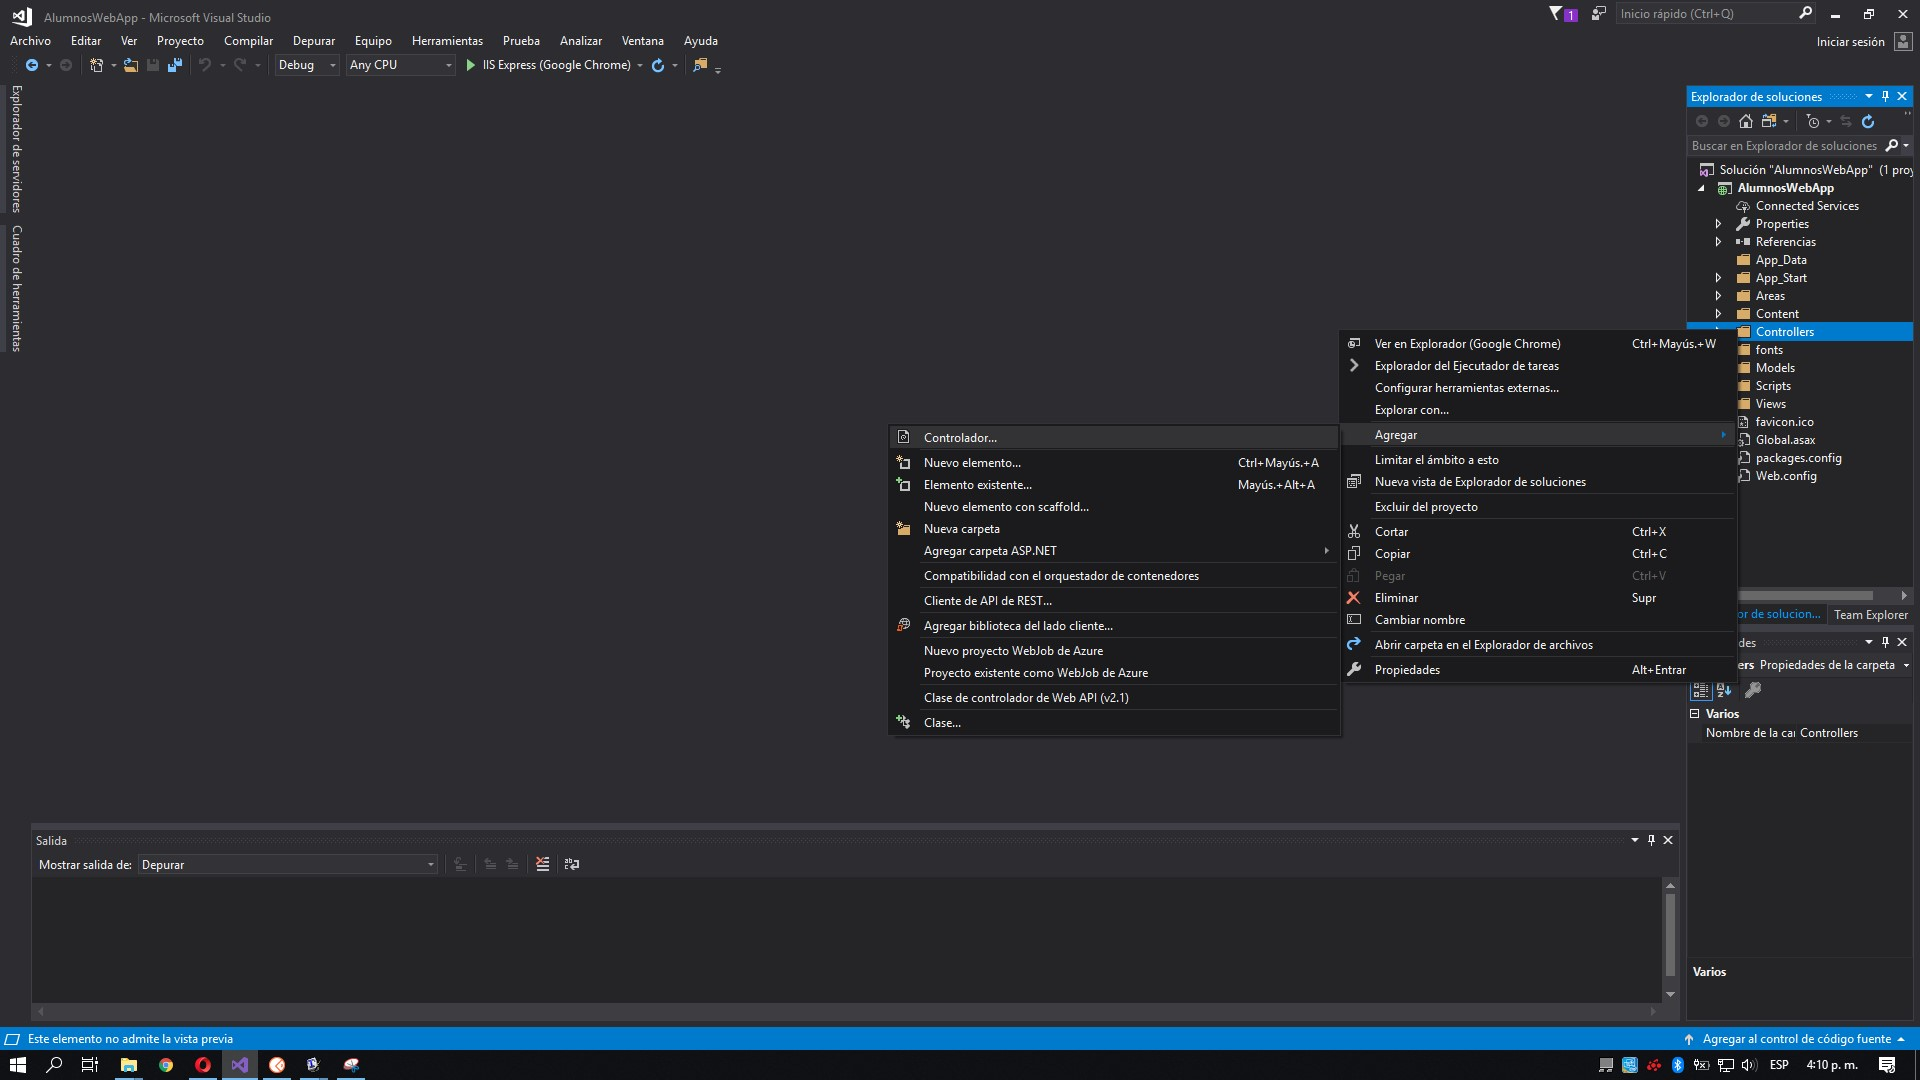
\includegraphics[width=15cm]{./Imagenes/Captura5}
	\end{center}
	\item Paso 7: En la ventana que nos aparece, Seleccionar la Opcion\\
	Controlador de Web API 2 con acciones que usan Entity Framework\\
	\begin{center}
		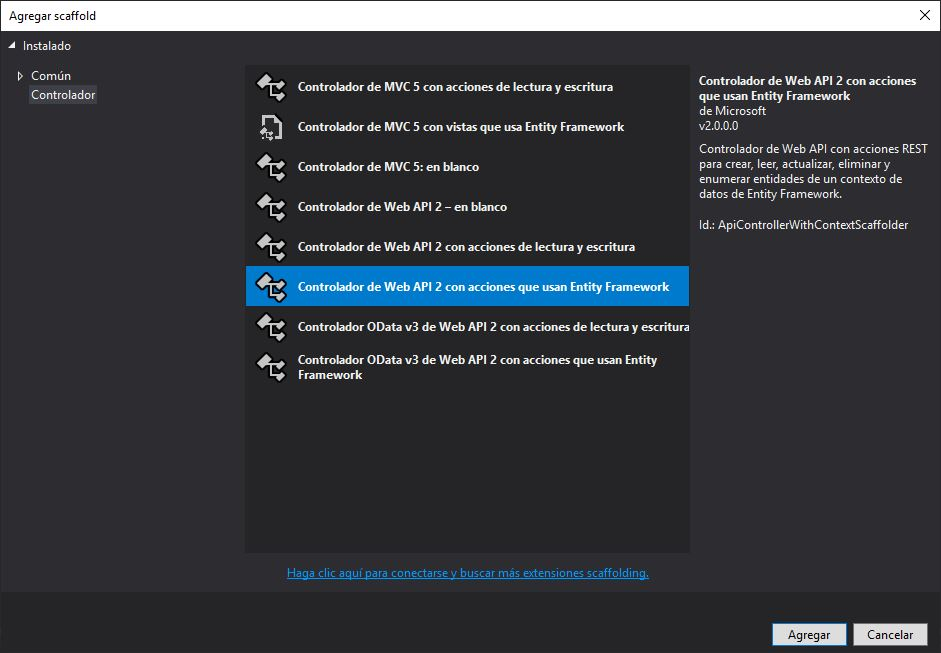
\includegraphics[width=15cm]{./Imagenes/Captura7}
	\end{center}
	\item Paso 8: Aparecerá una ventana para Agregar Controllador\\
	hacer lo mostrado en la imagen\\
	\begin{center}
		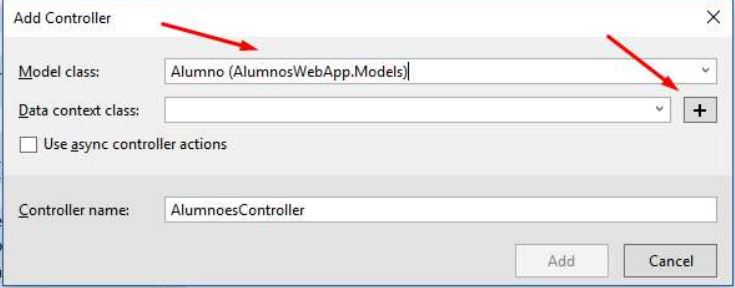
\includegraphics[width=15cm]{./Imagenes/Captura8}
	\end{center}
	\item Paso 9: Por defecto nos genera el nombre para el Nuevo Contexto de Datos, pulsamos Agregar o Add\\
	\begin{center}
		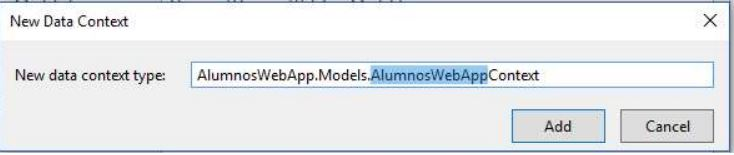
\includegraphics[width=15cm]{./Imagenes/Captura9}
	\end{center}
	\item Paso 10: Cambiamos el Nombre del Controlador de (AlumnoesController  a  AlumnosController) y Pulsamos Add\\
	\begin{center}
		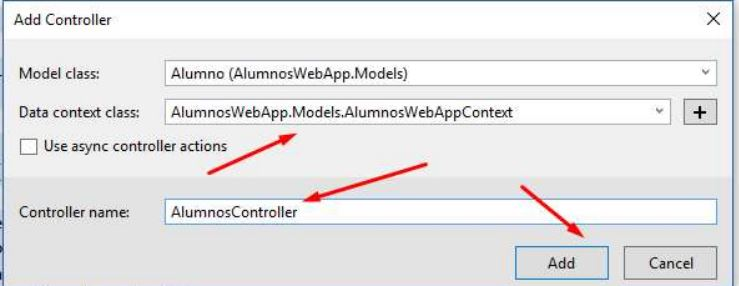
\includegraphics[width=15cm]{./Imagenes/Captura10}
	\end{center}
	\newpage
	\item Paso 11: Una vez creado el controlador AlumnosController\\
	Modificamos y agregamos condigo dentro de //GET: api/Alumnos\\
	\begin{center}
		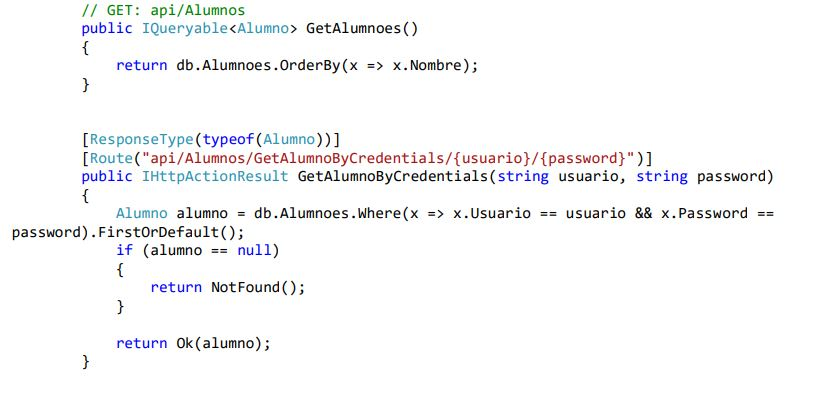
\includegraphics[width=15cm]{./Imagenes/Captura11}
	\end{center}
	\item Paso 12: Al igual que el anterior controllador, Agregamos un controlador nuevo llamado TareasController\\
	\begin{center}
		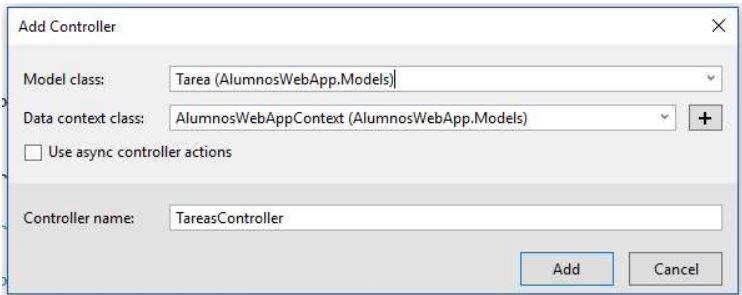
\includegraphics[width=15cm]{./Imagenes/Captura12}
	\end{center}
	\item Paso 13: Ahora dentro del controlador TareasController solo modificamos en // GET: api:Tareas  la linea (return db.Tareas)\\
	\begin{center}
		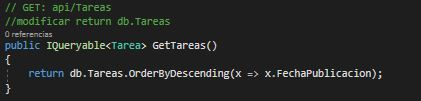
\includegraphics[width=15cm]{./Imagenes/Captura13}
	\end{center}
	\item Paso 14: Agregamos un ultimo controlador, Este se llamara TareaAlumnosController\\
	\begin{center}
		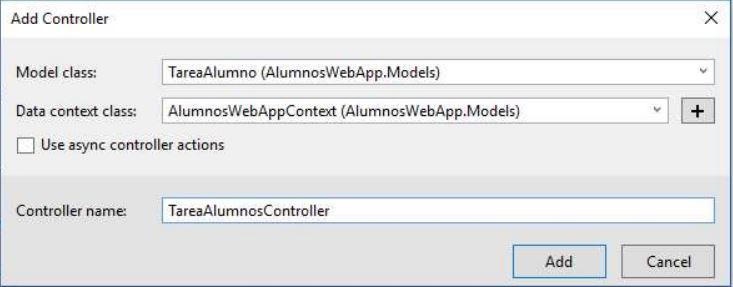
\includegraphics[width=15cm]{./Imagenes/Captura14}
	\end{center}
	\newpage
	\item Paso 15: Reemplazamos todo el código con las siguientes imagenes\\
	\begin{center}
		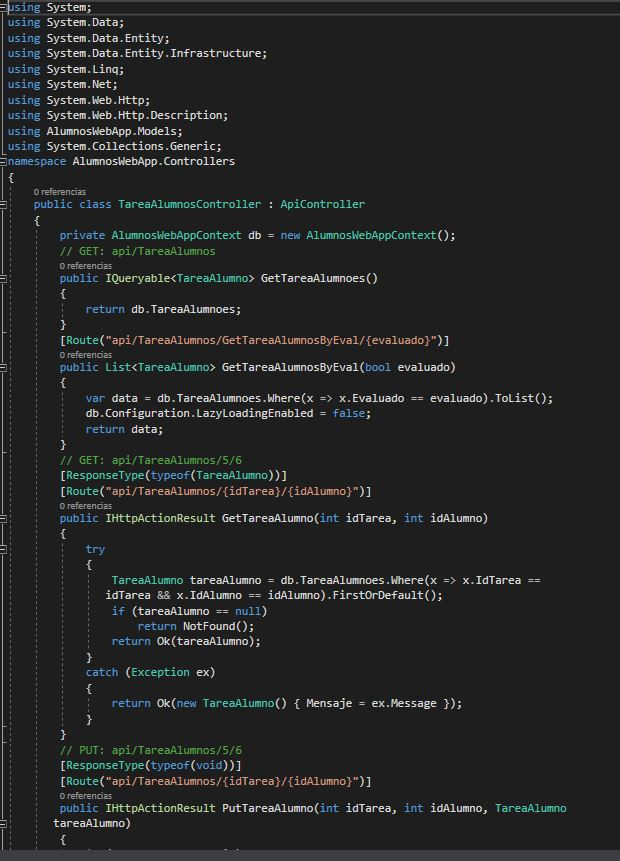
\includegraphics[width=15cm]{./Imagenes/Captura15}
		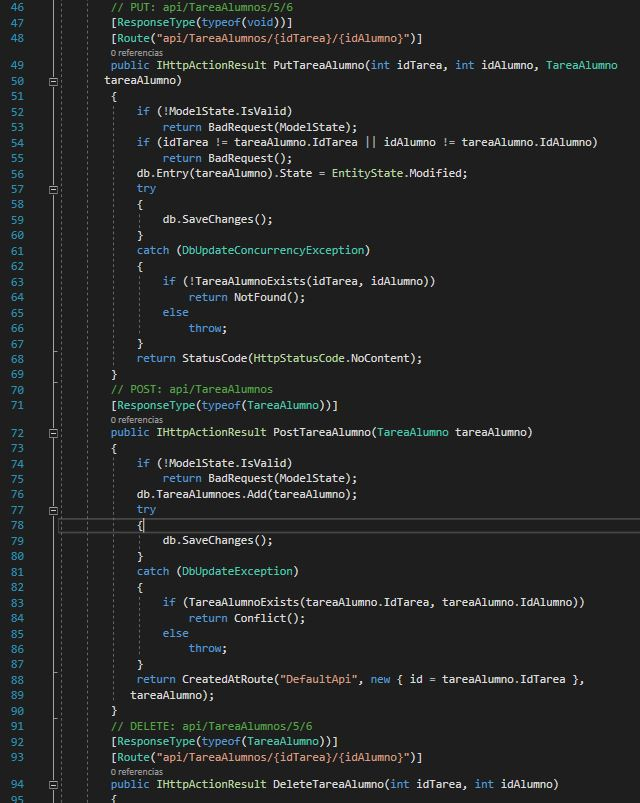
\includegraphics[width=15cm]{./Imagenes/Captura16}
		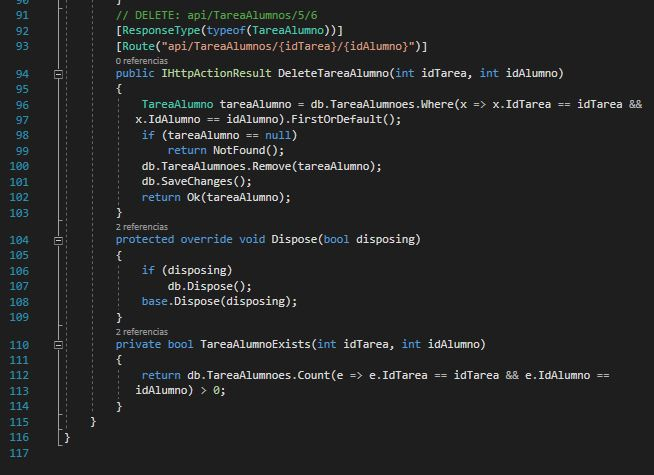
\includegraphics[width=15cm]{./Imagenes/Captura17}
	\end{center}
	\item Paso 16: Una vez terminado, Ejecutamos la solucion\\
	\begin{center}
		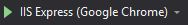
\includegraphics[width=15cm]{./Imagenes/Captura18}
	\end{center}
	\item Paso 17: Se abrirá un navegador (en este caso chrome) y debemos pulsar la opcion API\\
	\begin{center}
		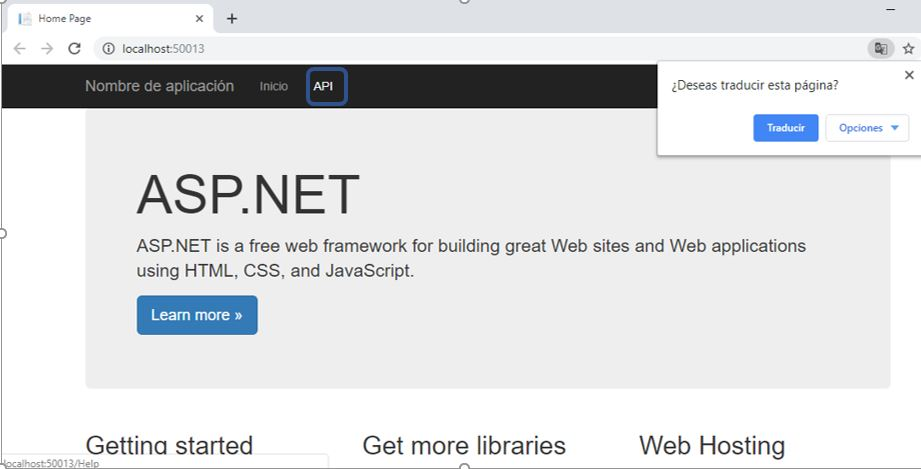
\includegraphics[width=15cm]{./Imagenes/Captura19}
	\end{center}
	\item Paso 18: Nos mandara a otra pagina en la que debemos buscar la opcion	(POST api/Alumnos) y la seleccionamos\\
	\begin{center}
		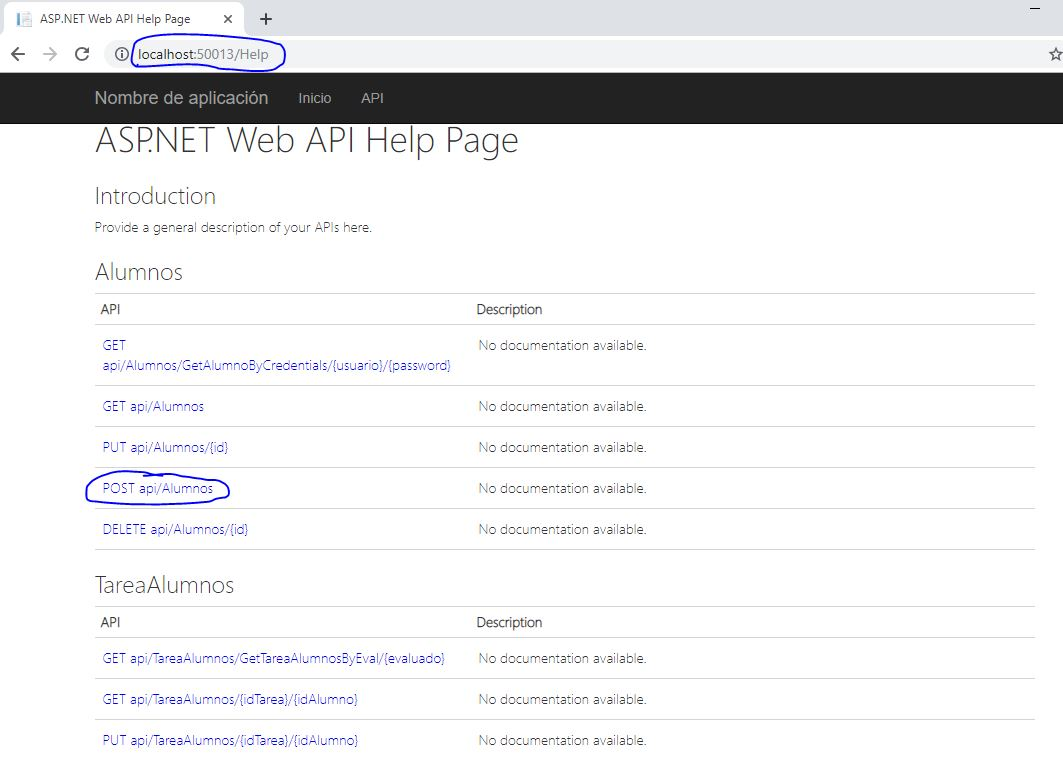
\includegraphics[width=15cm]{./Imagenes/Captura20}
	\end{center}
	\item Paso 19: Ahora hay que buscar un bloque de texto que se llame(application/json, text/json)\\
	Copiamos el ejemplo\\
	\begin{center}
		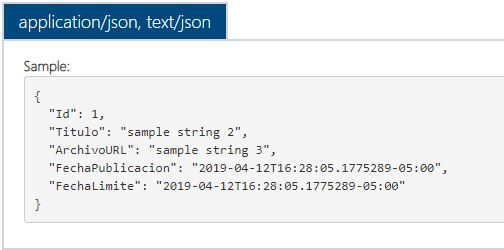
\includegraphics[width=15cm]{./Imagenes/Captura21}
	\end{center}
	\newpage
	\item Paso 20: Descargamos Postman, y lo instalamos, para luego dentro de postman abrimos una pestaña nueva dentro del mismo y hacemos lo siguiente\\
	\begin{center}
		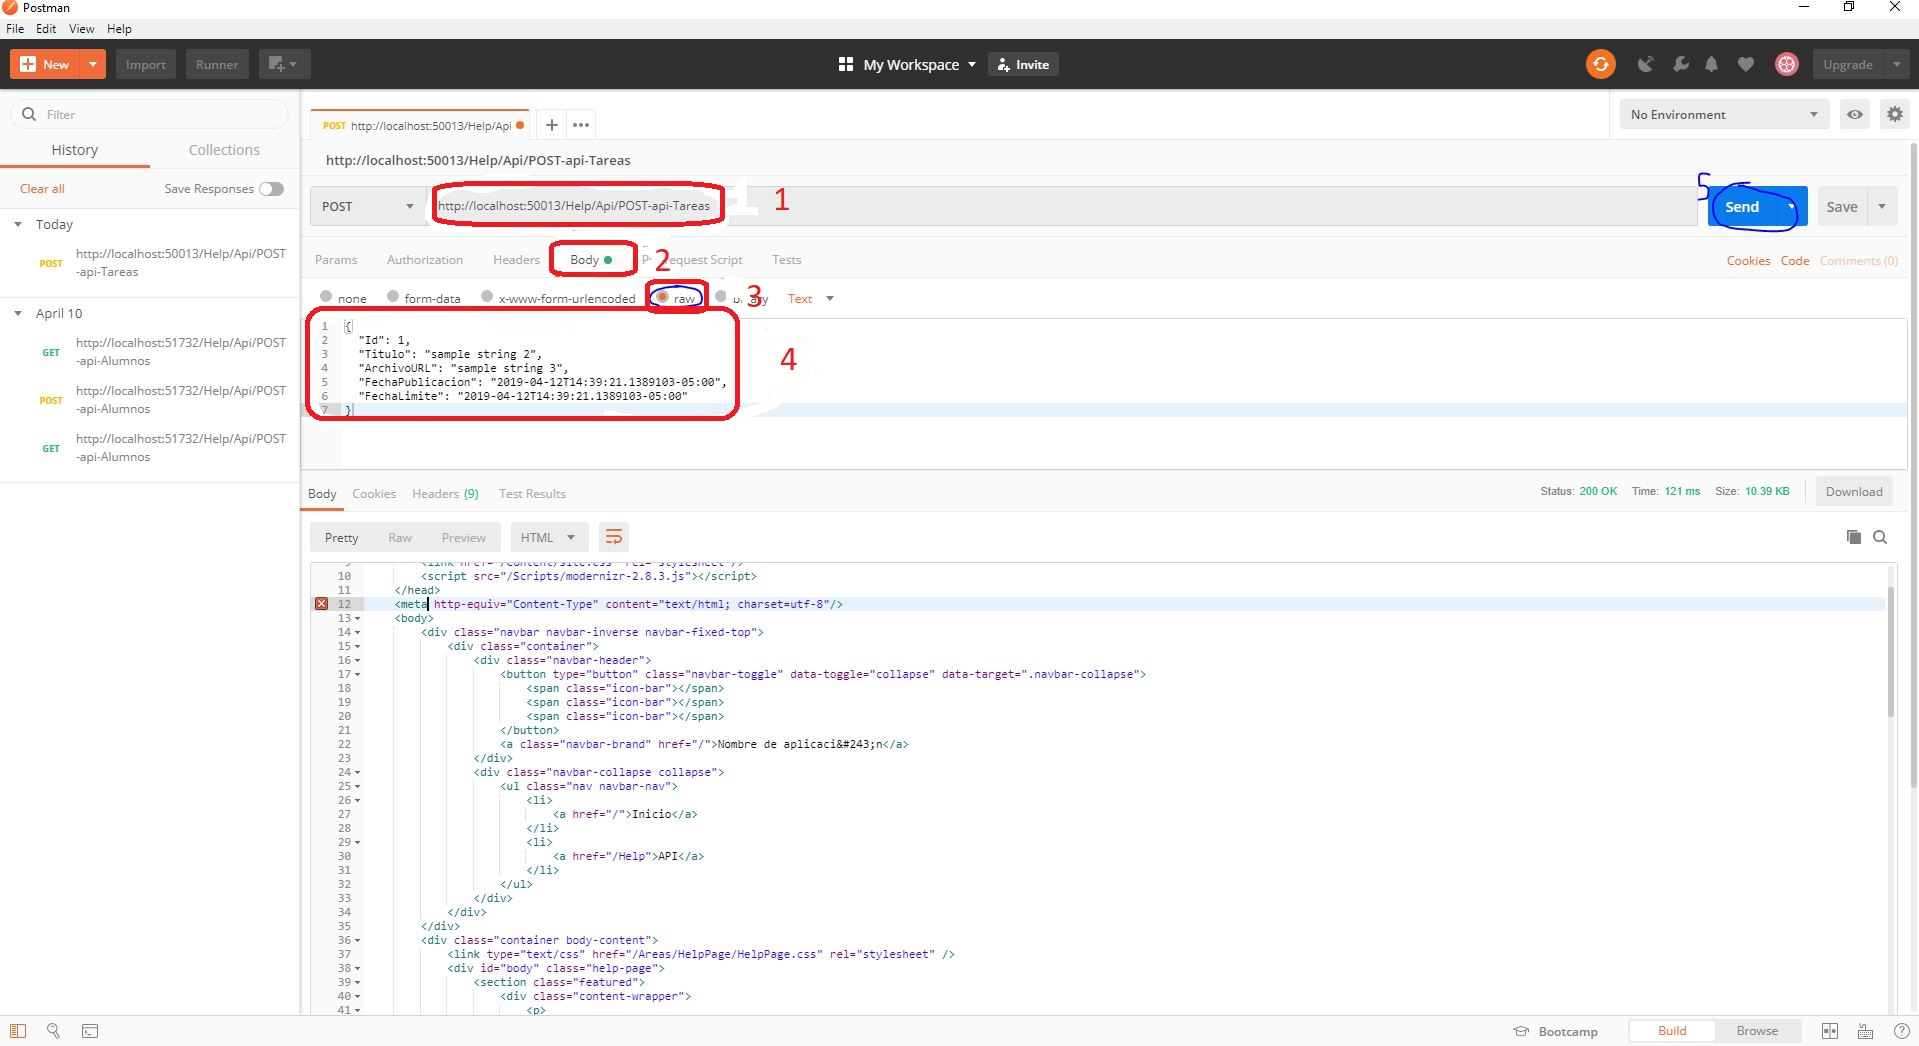
\includegraphics[width=15cm]{./Imagenes/Captura22}
	\end{center}
	
	
	
\end{itemize}






\section{ANALISIS E INTERPRETACION DE RESULTADOS} 
En el presente laboratorio se ha desarrollado un proyecto llamado "AlumnosWebApp" de tipo Web Application, usando la Web API para realizar con ello el servicio de REST.
Este proyecto trata acerca de calificar las tareas de los alumnos, haciendo primero el resgistro de los alumnos y sus tareas para luego relacionar las tareas con los alumnos correspondiente y de modo el cual se podrá poner una calificación.
Se utilizaron tres clases, una para la crecion del "Alumno" , otra para la creacion de la "Tarea" con sus respectivos atributos y otra clase de "TareaAlumno", que esta útima se llama al atributo de IdTarea y IdAlumno, aparte de sus atributos respectivos, para que se relacionen y se califique la tarea del alumno.
\\
Por medio de los controladores se usará la Web API por el cual podremos acceder a la web mediante el protocolo HTTP.
Una ves que tenemos el codigo listo, se para a verificar que el proyecto funcione con el servicio de Rest, que nos permiten listar, crear, leer, actualizar y borrar información.
Cuando solicitamos una pagina web, podemos hacer por diferentes métodos, el mas común es el GET, es el que usamos cuando digitamos una dirección en nuestro navegador, en ocasiones utilizamos POST, cuando enviamos un formulario con datos, pero las aplicaciones pueden usar otros métodos como PATCH, PUT, etc.
\begin{itemize}
\item Listar y leer: Usan el método GET
\item Crear: Usan el método POST
\end{itemize}
Para validar el funcionamiento, primero se ejecuta el proyecto y vemos observamos que formato de la cadena hay que seguir para probar en Postman, que es una herramienta que permiten realizar tareas diferentes dentro del mundo API REST. 
\begin{center}
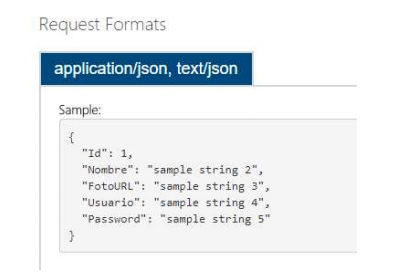
\includegraphics[width=5cm]{./Imagenes/analisis1}
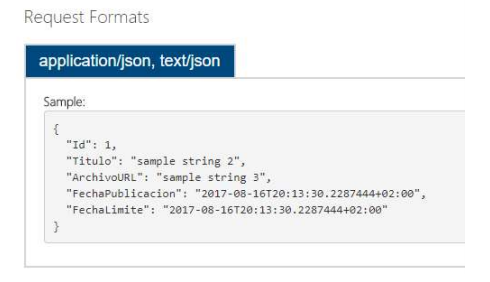
\includegraphics[width=5cm]{./Imagenes/analisis2}
\end{center}
Realizamos primero la creacion de un alumno, siguiendo el formato de la caden. Para crear un alumno usamos la operación de POST y para verifiCar si se ha creado el alumno, realizamos la operacion de GET; y lo mismo para el caso de la tarea.
Aqui se puede notar como se ha realizado correctamente el registro de ambos casos a través del servicio de REST y ahora lo que falta es vincular el alumno con su tarea y calificarla.
\\ Para realizar la calificación de la tarea del alumno se sigue la primera parte del formato de cadena y ahi se coloca tanto el indice del alumno como de la tarea y los datos correspondientes a la calificación, usando la operación de POST.
\begin{center}
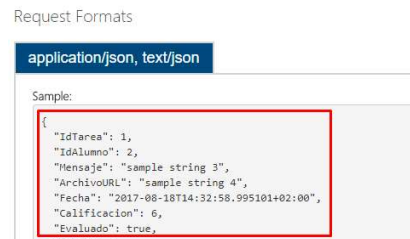
\includegraphics[width=5cm]{./Imagenes/analisis3}
\end{center}
Una vez realizada el registro de la calificación de la tarea del alumno con la operación GET podemos revisar si ha sido verdaderamente registrada. Gracias a estas operaciones de GET POST utilizadas la transferencia de datos en un sistema REST facilita la existencia de una interfaz uniforme que sistematiza el proceso con la información.
\section{CONCLUSIONES}

\begin{itemize}
	\item Usar el servicio REST Web Api, se pudo notar que necesita mas código para su implementación.
	\item El servicio REST se basa en conocer sobre HTTP.
	\item Nosotros hemos usado el formato JSON pero para la implementación de REST se puede usar cualquier tipo de descripcion.
\end{itemize}
\section{REFERENCIAS} 

American Chemical Society, 2005, Química. Un proyecto de la ACS. Ed. Reverté, Barcelona.

Atkins J. y Jones, L., 2012, Principios de Química. Los caminos del descubrimiento, 5ª Ed. Editorial Médica Panamericana, Madrid.

Chang, R., 2010, Química, 10ª edición, McGraw-Hill.

Masterton W.L., Hurley, C.N., 2003, Química: Principios y Reacciones. 4ª edición, Thomsom Editores, Madrid.

Petrucci R.H., Hawood W.S., 2003, Química general, 8ª edición, Prentice Hall


\end{document}
